\documentclass[11pt]{article}
\usepackage[T1]{fontenc}
\usepackage[utf8]{inputenc}
\usepackage[english]{babel}
\usepackage{amsmath,amssymb}
\usepackage{url}

\usepackage{pl-syntax/pl-judgments}

\title{15-791 ATPL \\ Week 11 Notes \\ Dependent Types Part 1}
\author{Jonathan Wilson}
\date{\today}

\begin{document}

\maketitle{}

\section*{Overview}

This week begins our talks of dependent types. There is little focus in this week on logical relations or proofs and rather an emphasis on language design. Part of this is due to there not being one single canonical form of dependently typed language and part of it is due to many dependently typed languages allowing beta reduction and in the type system which quickly becomes undecidable (not to mention the performance costs).

\section*{Review of Last week Call by push value}

Last week we covered partiality as well as other effects in Call-by-Push-Value (CBPV). In order to adapt logical relations to partiality, we needed a lemma called compactness. In short, compactness says that if a program terminates, it does so in some finite number of steps. 

Compactness: if force(susp$(x.C)) \mapsto^* ret(yes / no)$ then there exists an $n$ such that $force(susp^{(n)}(x.C)) \mapsto^* ret(yes / no)$

There exists other ways to deal with partiality including Denotational semantics however this only pushes the problem away from the operational semantics without providing us any tools to handle effects or effect-ful control flow. For this course, we prefer to stay lower level and focus on actual evaluation with operational semantics.

An alternative method that is a little more complicated but gives a little more insight into the problem is Pitts (spelling?). He uses a logical relation that is indexed by an upper bound on the number of steps that a program takes to terminate.

Logical relations on partiality rely on fixed point induction. This gives rise to methods of interpreting types as "complete denotational partial orders".
$$susp^{(0)}(x.C) \sqsubset susp^{(1)}(x.C) \sqsubset susp^{(2)}(x.C) \sqsubset \dots susp(x.C)$$
This gives rise to the mathematical interpretation of 
$$susp(x.C) = \sqcup_{i \ge 0} susp(x.C)$$
Where we can see a relationship between continuity (preserving limits) and termination. This works is a good solution for simple languages, but fails on higher order functions.

\section*{Introduction to Dependent Types}

Dependent type theory has roots as far back as intuitionistic logic itself. It is guided by types as propositions. Dependent type theory itself is credited to Martin-Lof. The four main primitive judgement of dependent type theory are:
\begin{align*}
    \Gamma \entails A type \quad & \Gamma \entails A \equiv A' type \\
    \Gamma \entails M : A \quad & \Gamma \entails M \equiv M' : A \\
\end{align*}
We not only have families indexed by some context gamma in the elements, but also the types. This implies that element-hood is inseparable from type-hood / type equality. There is no longer a phase distinction between the two. It is worth noting that term equality influences type equality as in 
$$\Gamma \entails Seq(7) \equiv Seq(7) type$$
relies on the equality of the term 7, but equality is syntactically incorrect for terms of two different types.

Typing is now Context Sensitive conciliations on well-formed programs. (well-formedness is now checked before types) 

Execution is still a transition system on states

Safety is still based on programs structured by types. We have some minimal sensibility conditions that apply before typechecking. After, types are special cases of structured constructors.

eg) list : Type $\rightarrow$ Type

"Type $\rightarrow$ Type" is a kind 

"list" is a constructor.

\subsection*{Aside: Pascal and dependent types in "boring" languages}

Pascal, a commonly cited and once widely used language that inspired the rise of object oriented programming, attempted a grossly simplified version of this by pulling some basic terms (i.e. constructors) into the their own kind through the use of singletons. Bob and PL paper denotes these singleton kinds $\mathbb{S}(3)$ or S(3), where 3 is just an example of a constructor. If you take HOT compilation, you will notice that this singleton kind calculus is one of many key insights for making a type preserving compiler for SML. This is necessary to handle the fact that modules influence the statics for SML yet functors and structs clearly have state and evaluation. 

My personal take is that practically all languages leverage at least the severely degenerate case of dependent types not just pascal. In C languages, arrays often degenerate into [ ] or even worse pointer types if you pass them into functions. However, arrays within a single function and even structs can be given a length [6]. This length must be known at compile time however showing the strict phase distinction of C. In pre C++-11 compilers, similar limitations exist. However, as of C++17, we now have constexpr functions which allow us to compute values at compile time (including the array type length) using basically anything in the language and getting more permissive every edition. This is shows ideas of dependent types have influences even on languages as far from the light of type theory as can be. In C++ circles, they have the same debates about how decidability is overrated as Bob had in class. It seems arbitrary to stop at decidable and not something like polynomial so we might as well allow any computation that can be done at compilation time (i.e., no user input). 

\subsection*{Families of types classify families of types}

What does it mean to have a family of types?

Well, we can think of our previous type systems as being a degenerate case of dependent type theory where the context is empty. 

$$\epsilon \entails 3 : nat$$

Whereas with elements in the context / families, we have:

$$x : Nat \entails Seq(2 * x) \equiv Seq(x + x) type$$

With families, we now wish to prove "functionality" of our types. Whereas before we could evaluate if two types are equal based on alpha-equivalence, we must now substitute in equal terms and prove.

If $M \equiv N : Nat$ then $Seq(2 * M) \equiv Seq(N + N) type$

While many people praise a specific form of dependent types, the most common form does not allow us to prove an equation as simple as the above. A more sensible view is to allow for any computation in the type system and ignore the problems of undecidability.

\subsection*{Weakening}
We would like the following to be true:
$$\Gamma x : A \Gamma' \entails x \equiv x: A$$
x is a derivation in the middle of the context however it still holds despite this.  We would like to maintain the invariant that if $\Gamma \entails M : A$, then $\Gamma \entails A type$. However, if we naively substitute from our x into the term we are type checking, our types may no longer make sense. Consider
$$\Gamma x : A, y : Seq(x) \Gamma' \entails (x, y) : A \times Seq(x)$$
\begin{center} \textbf{Incorrect Substitution:} \end{center}
$$\Gamma y : Seq(x) \Gamma' \entails (E, y) : A \times Seq(x)$$
Except in the second version, we no longer have a meaning for x in the context or in the type signature. To remedy this, we must substitute into the typing context that occurs after x, $\Gamma$' as well as the type signature
$$\Gamma x : A, y : Seq(x) \Gamma' \entails (x, y) : A \times Seq(x)$$
\begin{center} \textbf{Substitution:} \end{center}
$$\Gamma [E/x](y : Seq(x) \Gamma') \entails [][E/x](x, y) : [E/x](A \times Seq(x))$$
\section*{Second class on dependent type theory}
These four ideas are the core of dependent type theory: (Note: This material seems slightly different from the 5 key points on the official notes for this week. They might actually be the same though as there were two bullet points for number three at one point in the talk. Go check those out on page 3: https://www.cs.cmu.edu/~rwh/courses/atpl/pdfs/dependency.pdf)
\begin{enumerate}
    \item No entity without identity. i.e. equivalence judgments (that are equivalence relations) for both types and terms
    \item Congruence
    \[
    \frac{\Gamma \entails \theta(M_1, \dots, M_n) \quad \forall i \in [n], \Gamma \entails M_i \equiv M'_i : A_i}{\Gamma \entails \theta(M_1, \dots, M_n) \equiv \Gamma \entails \theta(M'_1, \dots, M'_n) }
    \]
    \item Invariance. Substitution and Weakening respectively
    \[
        \frac{\Gamma \entails M : A \quad \Gamma \entails A \equiv B}{\Gamma \entails M : B} \quad \frac{}{\Gamma x : A \Gamma' \entails x : A}
    \]
    \item Admissibilities. Different implementers do this diffferent, but the takeaways are the same.
    
    if $\Gamma \entails M : A$ then $\Gamma \entails A type$. This is a common presupposition when working with dependent type theory. It is similiar to the constraint that the context is well-formed.

    (NOTE: A Presupposition is something we wish to be true to make the proofs and theory easier, but instead of deriving from judgments each time we assert it, it must be true as a precondition.)

    If $\Gamma x : A \Gamma' \entails J$ and $\Gamma \entails M : A$ then $\Gamma [M / x] \Gamma' \entails [M/x]J$. The notation for J is confusing at first. J represents one of the four judgments that are core to dependent type theory. It could be a derivation that something is a type or a derivation that something has some other type.

    The same exact logic can be applied to equations. If $\Gamma x : A \Gamma' \entails J : B$ and $\Gamma \entails M \equiv N : A$ then $\Gamma [M / x] \Gamma' \entails [M / x] J \equiv [N / x] J: [M/x]B$
    
\end{enumerate}

In order to prove many properties about dependent type theory, we often need a strong lemma called Generalized Weakening. It is as follows.

If $\Gamma' \entails \gamma : \Gamma$ and $\Gamma \entails J$ then $\Gamma' \entails \hat \gamma (J)$

When proving either substitution or weakening, one must use the other one. This means the actual proof is quite involved. The issue arises when we try to invoke the IH when under the binder of a lambda. 

\section*{Predicativity and Universes}
When reasoning about logics, it can sometime arise that the definitions and application are circular. Martin-Lof made some of these mistakes when formalizing his type theory. This opened the way for Girard's paradox (I think the method is also vulnerable to Burali-Forti paradox). The solution to this is was developed by Whitehead and Russel. They developed a hierarchy of types all indexed by increasing natural numbers called cumulatively.

As this model is quite cumbersome to write and reason about, this gives rise to many languages adding tactics and the like as a type of metaprogramming to save the user time. Professor is not a big fan of prolific use of tactics as it often leads to much messier proofs when elaborated making it harder to reason about the actual proof underneath. It is partially for this reason we use Agda rather then a tactic based language.
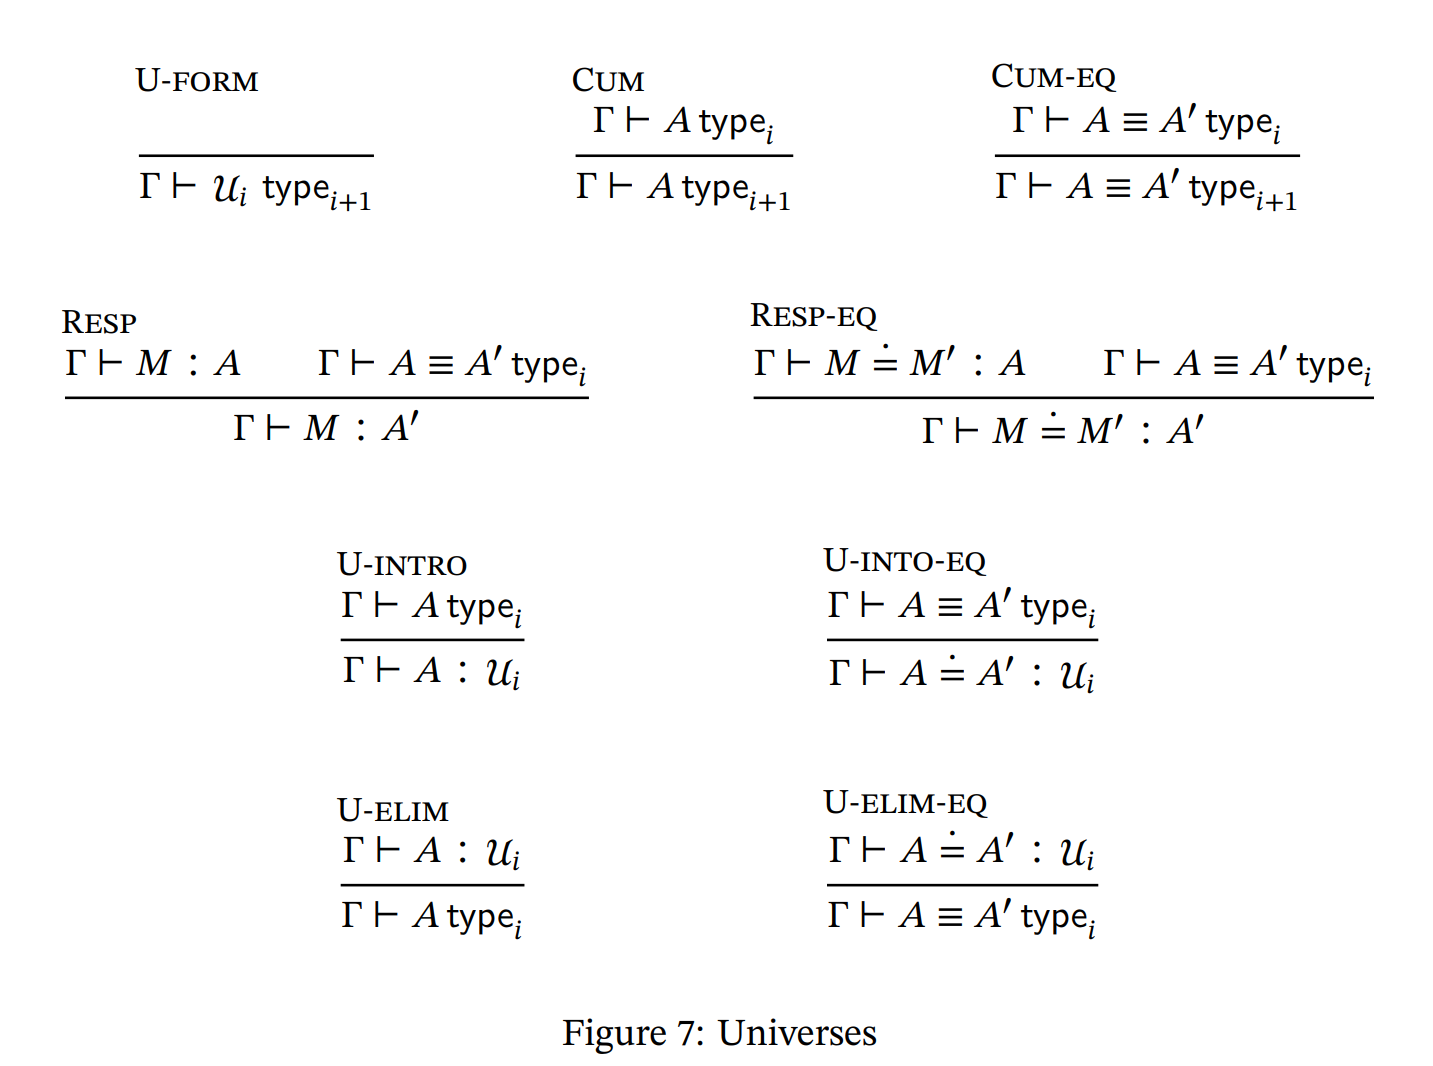
\includegraphics[width = \textwidth]{Universes.png}
This is directly from page 10 of the notes.

This is in contrast to an admissible cumulatively where the judgments are instead replaced with implications. A third choice common when subtyping is in play is to use subsumption rules often denoted with the symbol $\sqsubset$.

These things are related to the large cardinality axioms in set theory. In both these, we handle universes. This begins a discussion of how cardinality is not a useful metric in constructive logic. Bob mentions Cohen's power set of the naturals result and how you can generate seemingly endless subsets of the reals that are still the power set of the naturals. There is no canonical form then for these cardinality rules. Bob then finishes with a fun story about meeting Paul Cohen himself and the silliness of a set theory powered programming language.

\subsection*{Asides}
It was mentioned that the type theory internalizes judgment. This is similar to the interpretation of types over lambdas being related to uncurrying. $\Gamma \entails A \rightarrow B \cong \Gamma, A \entails B$
\section*{Using dependent types}
$$\frac{}{\text{bool type}} \quad \frac{}{true : bool} \quad \frac{}{false : bool} \quad \frac{\Gamma \entails M : bool \quad \Gamma \entails N : A \quad \Gamma \entails P : A}{if_{(A)} (M; N; P) : A}$$
Note that the notation (A) is only needed to assist in type synthesis. 
$$\frac{}{if(true; N; P) \equiv N : A}$$
$$\frac{}{if(false; N; P)  \equiv P : A}$$
$$\frac{}{if(M; true; false) \equiv M : A}$$
As in the notes, there is an argument over whether or not to include the induction principles for positive types like our boolean. While in one case they are valid substituting in for each branch and can allow us to derive true statements, they result in exponential blowup of our code. This has a relationship to solving binary decision diagrams and sat solving. Where we draw the line on what we want the computer to solve from here is blurry.
$$\frac{\Gamma \entails M : bool \quad \Gamma \entails N : A \quad \Gamma \entails P : A}{If(M; N; P)\text{ type}}$$
It is a bad move to derive that the if type has the uppercase If type as determining whether the two branches are indeed the same takes some serious proof. We want to still be able to say they have a common types if they are the same.
\subsection*{Dependent functions AKA Pi types AKA $\forall$}
$$\frac{\Gamma \entails A_1 \text{ type} \quad \Gamma, x : A_1 \entails A_2}{\Gamma \entails x : A_1 \rightarrow A_2 \text{ type}} \quad \frac{\Gamma \entails A_1 \text{ type} \quad \Gamma, x : A, \entails A_2 \text{ type}}{\Gamma \entails \lambda x . M_2 : (x : A_1 \rightarrow A_2)}$$
$$\frac{\Gamma \entails M_1 : (x : A_1 \rightarrow A_2) \quad \Gamma \entails M_2 : A_1}{\Gamma \entails ap(M_1, M_2) : [M_2 / x] A_2}$$
$$\beta - ap(\lambda x . M_2 , M_1) \equiv [M_1 / x] M_2 : [M_1 / x] A_2$$
$$\eta - \lambda x . ap (M, x) \equiv M : (x : A_1 \rightarrow A_2?)$$
Note: The official notes do not include parentheses around the Pi types, but I added them because the : operator is used for two different sorts of judgments.

As a matter of hygiene, we restrict our Pi types to only admit constructive proofs of existence. In other words, we cannot prove existence using $\neg \forall$.

\subsection*{How does dependency arise in the first place}
Equality types (or a better description is equality relations) are equivalent to propositional formulas. This is related to Church's Type Theory, but despite Church's overall brilliance, this type theory is very bad in Church's formulation. 
$$\frac{(\Gamma \entails A \text{ type})  \quad \Gamma \entails M, N : A}{\Gamma \entails M \equiv _A N}$$

$M \equiv _A N$ is formulated as $Id_A(M, N)$
$$\frac{\Gamma \entails M, N : A}{\Gamma \entails Id_A (M, N) \text{ type}} \quad \frac{\Gamma \entails M : A}{\Gamma \entails refl_A (M) : Id_A(M, M)} \quad \frac{\Gamma \entails M \equiv N : A}{\Gamma \entails refl_A(M) : Id_A(M, M)}$$
 
In other words, equality is defined as the least reflexive relation. The type Id internalizes our prior notion of equality.

Absolutely crazy induction rule for equality.
$$\frac{\Gamma, x, y : A, z : Id_A (x, y) \entails C type \quad \Gamma \entails p : Id_A(M, N) \quad \Gamma, x : A \entails Q : [x, x, refl_A (x) / x, y, z] C}{\Gamma J(M; xyz.Q) \quad _. [M, N, P / x, y, z] C}$$
Which leads to this equivalence
$$J(refl_A(M); x, y, z.Q) \equiv [M, M, refl_A(M) / x, y, z] Q : [M, M, refl_A(M) / x, y, z] C$$
At this point, class came to an abrupt end to be picked up next Thursday.

\end{document}